% In this last chapter an approach to the BCDI Phase Retrieval based on Automatic Differentiation will be discussed.
% It started from the necessity to 
% Unlke the DL model discussed above this method is iterative and

\epigraph{``An approach that would be superior to the ones considered here would be one that minimizes the Fourier-domain error while inherently satisfying the object-domain
constraints, or one that minimizes an error metric that combines the Fourier- and object-domain constraints [...]. 
Something along these lines would be very useful for the problem of a single intensity measurement; clearly, 
more could be done in this area''}{J.R.Fienup \cite{fienup_phase_1982}}

In this chapter a different approach to the BCDI phase retrieval will be presented. It originated from the need to resolve 
those cases in which neither standard alternating algorithms, nor the DL assisted PR can succeed to converge to a satisfactory 
reconstruction. The developed approach differs from the alternating projections algorithms classically used for 
the Fourier PR, as it is formulated as minimization problem solved with gradient descent (GD). The gradients however are computed 
through the efficient automatic differentiation (AD) enabled by graph-based differentiable programming packages like Tensorflow and 
PyTorch, accelerated on GPU. For this reason one could see the AD approach as unsupervised machine learning on a single training 
dataset.\\ 
The GD - based optimization is fundamentally different from fixed point alternating projections. Here one could qualitatively say 
that if the latter switches between real and reciprocal space applying constraints in both, the former initializes a 
complex object and updates at each cycle its modulus and phase using the gradients, with respect to them, of the differences 
between the observed and calculated diffracted intensities. In this way, the knowledge on the particle can be implemented 
by initializing the object with some physical constraints or adding regularization terms that will drive the updates 
towards more reasonable solutions. \\

% After mentioning the most relevant literature on AD, and more generally GD-based, phase retrieval for CDI, 
% we will present our formulation of the problem and the results obtained on simulated and experimental BCDI patterns. 

\section{State of the Art}
AD methods for PR have been investigated already in 2014 by Jurling and Fienup \cite{Fienup_AD} who first considered the use of 
AD for GD-based PR. In this theoretical work the authors proposed a pedagogical ``manual automatic 
differentiation'' approach for the phase problem, extended to complex-valued variables. The authors also denounced the 
lack of suitable softwares as major limitation to the use of AD-based PR. The advent of high-level, GPU oriented, libraries such 
as Tensorflow, PyTorch, JAX and Autograd has opened the opportunity to efficiently exploit AD algorithms for the phase problem. 
The first implementations in the CDI field have considered mostly ptychography in forward and Bragg geometries \cite{Nashed_2017, Kandel_2019} 
and multi-Bragg CDI \cite{Maddali_2023}. Chronologically, it was firstly Nashed and coauthors in 2017 \cite{Nashed_2017} 
who opened the field using a Tensorflow AD model for ptychography using the ADAM optimizer. From the same group, Kandel 
\textit{et al.} in 2019, showed the competitive performance of the AD model when compared to conventional algorithms and 
extended the model to multi-angle Bragg ptychography on simulated data. In 2023 Maddali and coauthors \cite{Maddali_2023} explored 
the use of AD methods for multi reflection Bragg CDI. The authors leverage the flexibility of the GD approach by designing a global 
optimization function that simultaneously accounts for the geometrical and physical constraints related to multi reflection 
BCDI. More recently Zhou in 2024 \cite{Tagaki_2024} and Wu in 2025 \cite{tagaki_2025} developed AD-based PR algorithms that 
are able to reconstruct large particles, for which a dynamical description of the scattering processes is required. These 
works again exploit the flexibility of AD-based models for the implementation of a forward model tailored to the specific 
problem of mixed kinematic and dynamic x-ray scattering taking place in large crystals. 

At the moment of writing, there aren't any published works that aim at solving the phase problem for hardly invertible BCDI 
datasets.

\section{Model implementation}
In an AD-driven optimization problem some trainable parameters are initialized. In the first basic formulation these 
trainable parameters can be the values of the voxels corresponding to the modulus $m$ and the phase $\varphi$ of the complex objects 
that represents the solution of the PR problem. All of these voxels contribute to the creation of a simulated 
diffracted intensity pattern via the forward model $I_{calc} = |\mathcal{F}\left\{ me^{i\varphi} \right\}|^2$. Subsequently, 
the gradients of a metric (loss function) that estimates the distance between the observed BCDI pattern $I_{obs}$ and $I_{calc}$ are calculated 
with respect to each of the trainable variables with automatic differentiation. At this point the value of each of these voxels is 
updated using a chosen optimizer (SGD, ADAM, etc.) and a given learning rate. The Tensorflow library allows for an easy 
implementation of the trainable variables and loss function and handles gradient operations with predefined methods. It is therefore 
straightforward to run the optimization as it follows the same structure of a deep learning model, with less trainable parameters and 
for a single data. 

However, such simple formulation of the complex object as mere real-valued variables is not optimal for a non-linear and non-convex 
inverse problem such the Fourier phase retrieval. In fact, many non-physical modulus-phase configuration could yield a 
$I_{calc}$ that is close to  $I_{obs}$. The presence of these local minima is the reason why, in conventional PR, algorithms 
like hybrid input-output, capable of escaping them, are employed. 
Moreover, it was shown by Marchesini in \cite{marchesini_unified_2007}
that steepest GD and even more sophisticated conjugate GD are more prone to get stuck in local 
minima, reason why they are not commonly utilized for Fourier PR. However, the active research field of machine learning has 
brought important advancements in the formulation of efficient and robust optimizers based on stochastic gradient descent with 
powerful features like Nesterov or adaptive momentum (ADAM \cite{ADAM}). These GD techniques are more robust to local minima, 
since the gradient is computed on mini-batches of trainable variables rather all of them (stochastic rather than classical steepest GD), 
and converge faster thanks to the ``memory'' of previous steps. Additionally, they are often wrapped into handy classes, ready to use, 
in Tensorflow and Pytorch libraries.  

However, to facilitate the convergence the formulation of the complex object to be optimized has embedded some physical considerations that 
helped to restrict the solution space. First of all, both support and phase built on a 3D grid occupying half the volume of the 
input BCDI data to account for the oversampling ratio which has to be at least 2 in all directions to ensure invertibility.  
Additionally, other constraints specifically designed for the object shape and phase were considered. 

\subsection{Object's shape}

The formulation of the object's shape has started considering the typical crystalline samples that are studied with the BCDI technique
and the requirements the modulus of the reconstructed object need to fulfill to be considered a ``good solution''. 
Usually, successful reconstruction show a \textit{homogeneous} modulus, sometimes quantitatively assessed through the 
mean-to-max metric \cite{Frisch2023CuAgCatalysts} , \cite{Grimes2024CatalystStrain}, as in standard BCDI the form factor is 
approximated uniform across all the scattering sites. Enforcing a homogeneous modulus by construction limits the search space 
and helps the convergence to the solution \footnote{This approach of constraining the modulus of the object to be homogeneous was already 
considered in the literature (see \cite{madsen2021})}.
It follows that parametrizing the \textit{surface} of the support, and setting to 1 the inside, is much more advantageous than optimizing 
the full 3D volume. This approach, already proposed by Scheinker and Pokharel in \cite{scheinker_adaptive_2020}, 
also significantly reduces the number of variables to optimize.

An additional consideration is that the probed samples are crystalline, thus often \textit{faceted} and \textit{convex}. 
Therefore, one could simplify even more the construction of the object shape by building a certain amount of planes in the 
3D space and obtain the support from the volume that lies inside the intersections of all them. This would remove the possibility 
to have spikes or rough surfaces that might satisfy some local minimum but wouldn't represent a crystal. Moreover, with this 
representation the number of trainable variables would be further reduced. 

According to this scheme the relevant parameters to be optimized are the angles $\theta$ and $ \varphi$ of the spherical 
coordinates and the length $d$ of a given number $N$ of the so-called \textit{half-spaces}. 
More formally, the normals $n_i$ for each of the $N$ half-spaces are defined with a pair of ($\theta , \varphi$) that  its
orientation in space (Eq. \ref{eq:normal_vector}). Subsequently, only the intersection of those $(x,y,z)$ coordinates for which the dot product with 
each $n_i$ is smaller than the length $d_i$ is considered as support (Eq. \ref{eq:convex_hull}).


\begin{equation}
    \mathbf n_i \;=\;
    \begin{pmatrix}
    \sin\varphi_i\cos\theta_i \\[6pt]
    \sin\varphi_i\sin\theta_i \\[6pt]
    \cos\varphi_i
    \end{pmatrix},
    \label{eq:normal_vector}
\end{equation}
    
\begin{equation}
    \mathcal S \;=\;
    \bigcap_{i=1}^N
    \Bigl\{\mathbf x=(x,y,z)\in\mathbb R^3 : 
    \mathbf n_i\cdot\mathbf x \le d_i\Bigr\},
    \label{eq:convex_hull}
\end{equation}

A schematic representation of this construction is provided by Fig. \ref{fig:support_construction}.
 
With this approach the user needs to provide a number of half-spaces as hyperpareter meaning that a sort of prior knowledge 
on the sample can be leveraged in these regards as well. However, this number doesn't have to be precisely the number of 
facets expected. In fact, a large $N$ is often advised for unknown sample shape such that even roundish objects can be 
retrieved. In case of well faceted samples the large $N$ is a minor problem as many $n_i$ will be automatically aligned to the 
same $(\theta_i, \varphi_i, d_i)$ at the cost of some more trainable parameters. 

The first drawback of this convex-hull parametrization is that concave objects can't be retrieved. However, these cases 
are much less frequent in typical BCDI experiment. The second limitation is that this formulation is incapable of modeling 
defects that would zero the contribution of the object's modulus to the diffraction pattern \cite{favre-nicolin_analysis_2010}. 
A correct BCDI reconstruction of particles affected by this type of defects presents ``holes'' inside the hull in correspondence of the 
defect. However, the current model cannot address this type of features as the support is by construction fully homogeneous 
inside the borders. Further developments of the algorithm could indeed aim at a more complete formulation of the construction 
of the object modulus. 

\begin{figure}[H]
    \centering
    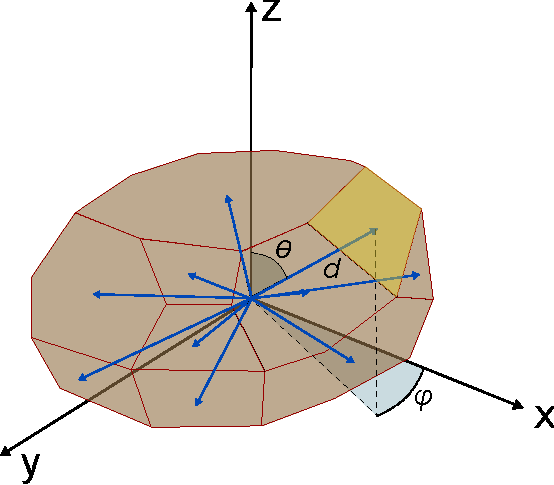
\includegraphics[width=.8\textwidth]{figures/AD/AD.pdf}
    \caption{Construction of the convex hull with half-spaces expressed with spherical coordinates }
    \label{fig:support_construction}
\end{figure}

The last important consideration of this parametrization is that the support $\mathcal S$ is sharply divided into a binary 
variable (1 inside and 0 outside) thus leading to differentiability problems. In fact, in such a way the gradients, essential for the 
support update, are not defined. For this reason $\mathcal S$ is first passed through a sigmoid function controlled by a
hyperparameter $\epsilon$ responsible for the smoothening of the support borders. This measure can also be seen as a control of the 
resolution of the object. Additionally, a mildly steep sigmoid in the early stage of the optimization can function help retrieving 
a low resolution estimate of the support, that can be further refined adjusting the $\epsilon$ parameter. \\

\subsection{Object's phase}
The parametrization of the object's phase is more challenging. From a qualitative point of view, the prior knowledge 
that can be exploited for a tailored implementation, is limited to the awareness that a physically meaningful atomic displacement 
field cannot have ``too many'' sharp variations. This observation is translated into code by smooth functions parametrization or total 
variation (TV) regularization of the object's phase. While the former would enforce smoothness by construction the latter 
would operate adding a penalty to the data-fidelity term of the loss function for non-smooth solutions. Both approaches have been 
explored and are here reported. \\

Forcing a scalar field defined on an  $L\times H\times W$ grid to exhibit smooth behavior is equivalent to seeking a 
sparse representation of that field—that is, to concentrating its essential information into far fewer degrees of freedom 
than the original $L\times H\times W$ samples. 
Concretely, one looks for a change of basis in which the field can be written as a linear combination of a hierarchy 
of modes or atoms, ordered by “importance.” In a Fourier or wavelet expansion, for instance, the expansion coefficients 
are naturally sorted from largest (low‑frequency or coarse‑scale modes) to smallest (high‑frequency or fine‑scale modes). 
Retaining only the largest coefficients both compresses the data and removes rapid oscillations, yielding an inherently 
smoother reconstruction. Equivalently, in the matrix case a Singular Value Decomposition (SVD) identifies an orthonormal 
basis in which only a few singular values are nonzero; by truncating to the top singular values one obtains a low‑rank 
— and thus smoother—approximation \cite{golub1996matrix}. For higher dimensional data, this same principle underlies 
higher-order generalizations of the SVD—Tucker/HOSVD, CP, Tensor-Train, and T-SVD—each of which orders multilinear 
“modes” by their singular-value (or eigenvalue) strength, and truncating to a small subset produces both compression 
and smoothness \cite{Kolda_TT}. 

In this case the Tucker decomposition was chosen, among the several possible methods, for its simplicity of implementation 
with the Tensorflow library and for the suitability for moderately low dimensions \cite{Oseledets_TT}. 
For a 3D tensor the Tucker decomposition is done as follows: 

Considering \(\mathcal{\varphi} \in \mathbb{R}^{L \times H \times W}\) the 3D object's phase. The Tucker decomposition expresses \(\mathcal{\varphi}\) as:
\[
\mathcal{\varphi} = \mathcal{G} \times_1 U^{(1)} \times_2 U^{(2)} \times_3 U^{(3)},
\]
where:
\begin{itemize}
  \item \(\mathcal{G} \in \mathbb{R}^{R_1 \times R_2 \times R_3}\) is the \textbf{core tensor},
  \item \(U^{(1)} \in \mathbb{R}^{I \times R_1}\), \(U^{(2)} \in \mathbb{R}^{J \times R_2}\), and \(U^{(3)} \in \mathbb{R}^{K \times R_3}\) are the \textbf{factor matrices},
  \item \(\times_n\) denotes the mode-\(n\) tensor-matrix product.
\end{itemize}

In index notation, this becomes:

\[
\mathcal{\varphi}_{i,j,k} = \sum_{\alpha=1}^{R_1} \sum_{\beta=1}^{R_2} \sum_{\gamma=1}^{R_3}
\mathcal{G}_{\alpha,\beta,\gamma} \cdot U^{(1)}_{i,\alpha} \cdot U^{(2)}_{j,\beta} \cdot U^{(3)}_{k,\gamma}.
\]

With this formulation the parameters $R_1, R_2, R_3$ are set by the user and define the ``storage space'' in which the 
information required to represent $\varphi$ has to be condensed. It is proven that for $R_i = L,H,W$ respectively, the 
tensor $\varphi$ is exactly represented. However, being the goal a spare representation of the object's phase these numbers 
are chosen significantly smaller than any of the sizes of the array. The Tensorflow implementation of the Tucker decompostion 
is rather straightforward as the function \texttt{tf.einsum()} takes care of the tensor contraction.\\

A different approach that has been considered, leverages the TV regularization to push the algorithm towards a smooth object's 
phase. The full $L\times H\times W$ tensor is therefore optimized and a penalty on the sum of the absolute value of the 
gradients of the phase is added to the loss function. Precisely, the formula that has been used calculates the sum of the 
\textit{squared} gradients, since the square root operation, necessary to obtain the correct formula, creates 
problem around zero because of the infinite gradient. The final equation is therefore: 

\begin{equation}
\centering
   TV =  \alpha \sum_{i = 1}^{L}\sum_{j = 1}^{H}\sum_{k = 1}^{W} \mathcal S[(\varphi_{i} - \varphi_{i-1})^2 + \varphi_{j} - \varphi_{j-1})^2 +  \varphi_{k} - \varphi_{k-1})^2]
\end{equation}

where $\alpha $ is a hyperparameter that acts as a scaling factor, $(i,j,k)$ are the indices running over the coordinates of
the $L\times H\times W$ grid and $\mathcal S$ is the object support. The parameter $\alpha $ in this case was chosen to be assigned as a fraction, imposed by the user, 
of the value of the data fidelity loss. Further developments could aim at finding adaptive formulations for the magnitude 
of $\alpha $. 

\subsection{Loss function}
Another important aspect of the model is the loss function. Typically, for inverse problems there is a \textit{data fidelity}
term that in this case measures the distance between $I_{obs}$ and $ I_{calc}$ according to some metric, and other additional 
\textit{regularization} terms that guide the optimization process with physical constraints. 

\textbf{Data fidelity}: 
The most common and intuitive metrics are the Mean Squared Error (MSE) and the Mean Absolute Error (MAE) that evaluate 
the Euclidean distance between the observed and calculated intensities. Practically, because of the large dynamic range 
of typical BCDI data, the MAE performs better as it doesn't focus on bright pixels only, but manages to correct for lower 
intensity tails as well. 
A more faithful metric for BCDI experimental data is the Poisson Negative Log-Likelihood (P-NLLK). This metric assumes 
indeed the handling of count data, like the type obtained by photon counting detectors, and that the stochasticity of physical 
process is Poisson distributed. When summed over the full dataset, the discrepancies between calculated and observed 
intensities are not intended as Euclidean distances but like divergences between two probability distributions. In other 
words, the P-NLLK estimates the likelihood that $I_{calc}$ belongs to the same Poisson distribution of $I_{obs}$ \cite{Thibault_2012}. 
Derived from the equation for the probability for Poissonian events, the formula of the averaged P-NLLK, in the form of 
a Kullback-Liebler divergence is: 

\begin{equation}
    \bigl\langle \mathrm{P-LLK}\bigr\rangle
    = \frac{2}{N_{\mathrm{obs}}}
    \left[
      \sum_{I_{\rm obs}>0}
        \bigl(
          I_{\rm calc} - I_{\rm obs}
          + I_{\rm obs}\,\ln\!\frac{I_{\rm obs}}{I_{\rm calc}}
        \bigr)
      \;+\;
      \sum_{I_{\rm obs}=0} I_{\rm calc}
    \right].
\end{equation}
    

Both the MAE and the P-NLLK have been tested on several simulated and experimental datasets and the MAE has always shown 
better convergence. An explanation for this unexpected result is yet to be found, but the main suspect is that the gradients 
calculated during the backpropagation can have instabilities because of the logarithm. 

\textbf{Regularizations}:
Beside the TV on the object's phase to ensure smoothness, another term that was considered concerns the size of the support. 
For a given data fidelity value, it is known that the object with the smallest support represents the optimal solution 
\cite{favre-nicolin_free_2020}. Intuitively this could be explained with the fact that there are many more object phase configuration 
that would combine constructive and destructive interferences to match the observed intensity in reciprocal space. 
The analogous measure is the shrinkwrap algorithm \cite{Marchesini_shrinkwrap} utilized in alternating projections algorithms.  
For this reason a penalty $P$ on the size of the support can be added to the loss function with the formula: 

\begin{equation}
    \centering
    P = \beta  \sum_{i,j,k} \mathcal S
\end{equation}

where $\beta$ is a hyperparameter that similarly to $\alpha$ is chosen by the user with respect to the data fidelity loss. 
Both the hyperparameters can be tuned manually during the optimization, to adjust in case of need, the strength of 
the regularization terms. 
The final formula for the loss function can be ultimately expressed as: 

\begin{equation}
       L = \frac{1}{N_{\mathrm{obs}}}
       \sum_{i=1}^{N_{\mathrm{obs}}}
       \bigl\lvert I_{\mathrm{calc},i} \;-\; I_{\mathrm{obs},i}\bigr\rvert  
        + \alpha TV(\varphi)
        + \beta  P(\mathcal S)
\end{equation}

For the optimization, a tolerance on the MAE value or a fixed number of steps can be set to stop the algorithm. Empirical 
observations have shown that a MAE value around 0.2 is sufficiently low for the result to be considered good. However, 
an additional refinement with a few iterations ($\sim$ 300) is recommended for cross-validation.  \\

Before concluding the paragraph, it is worth highlighting that this AD implementation offers the possibility to simultaneously 
run multiple reconstructions in parallel, efficiently on the GPU. One can create a 4D tensor by stacking several copies of the 3D 
intensity data, creating therefore a batch. For each element in the batch a different initial support and phase configuration 
can be chosen, hence increasing the likelihood to converge to the solution. 

\section{Results}
In this section two relevant results will be presented. The first examples is a highly strained Palladium particle on 
measured at the ID01 beamline of the ESRF \cite{bellec2026ultrafast}. 
The large strain inside the particle distorts the BCDI pattern and makes the reconstruction with conventional iterative 
algorithms overly challenging. 
% This dataset has been measured with the novel Bragg Coherent Modulation Imaging (BCMI) technique that yielded excellent 
% result, presented as ground truth reference. 

\subsection{Hardly-invertible BCDI patterns with high strain}

\begin{figure}[H]
  \centering
  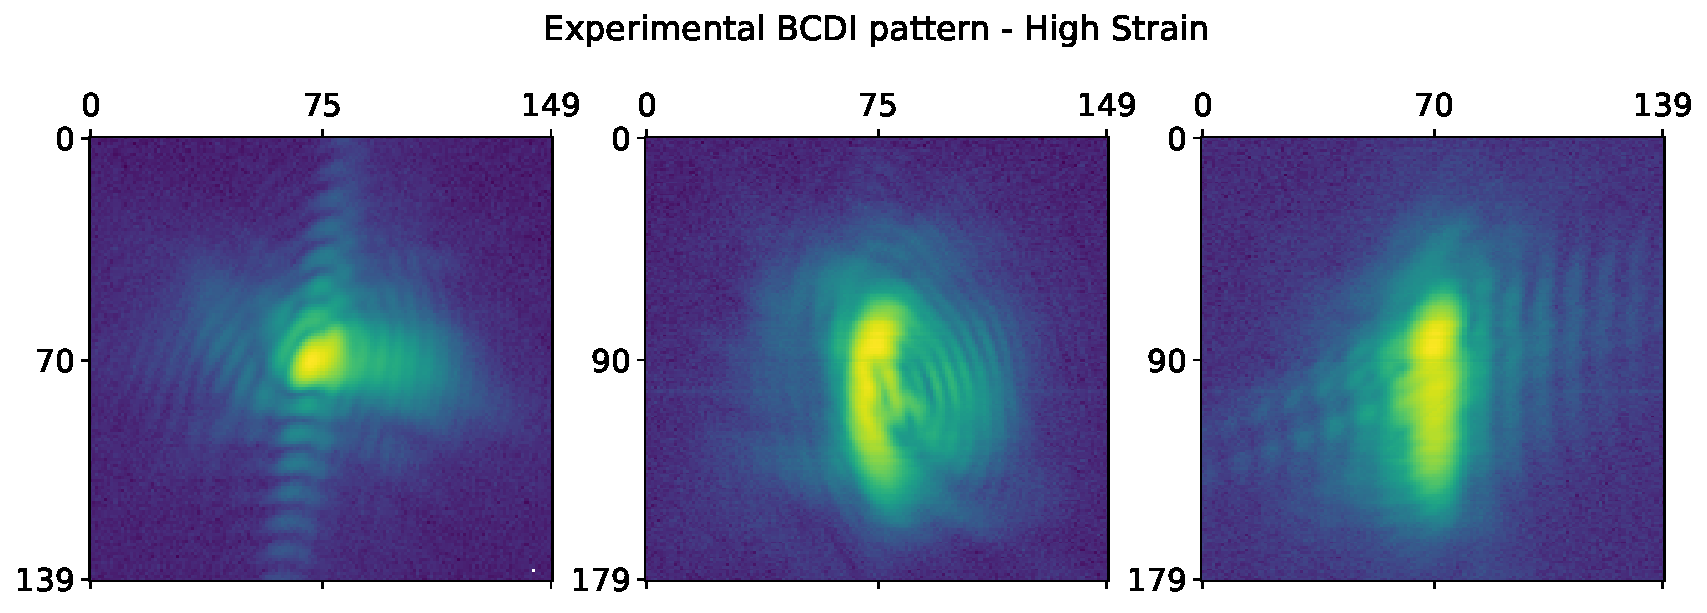
\includegraphics[width=\textwidth]{figures/AD/AD_exp3_michael.pdf}
  \caption{Projections along the three axes of a BCDI pattern of the highly strained Nickel particle. }
  \label{fig:projections_michael}
\end{figure}

In the following lines a comparison between different reconstruction methods will follow. Namely, (i) the results obtained 
from 40 independent runs of standard PR using PyNX software. Each run consisted of 400 HIO iterations followed by 1000 RAAR and 
300 ER ones. The parameters of are displayed in Table \ref{table:pynx}. 
At the end of the process, the two best reconstructions among the 40 runs according to the ``mean to max'' metric \cite{Frisch2023CuAgCatalysts, Grimes2024CatalystStrain} 
are combined using the mode decomposition technique proposed in \cite{favre-nicolin_free_2020}. 
This method is referred in the text to as ``PyNX''. 

\begin{table}[H]

  \centering
  \resizebox{\linewidth}{!}{%
    \begin{tabular}{|l|l|}
      \hline
      \textbf{Parameter} & \textbf{Value} \\
      \hline 
      \texttt{recipe}                                  & \texttt{400 HIO + 1000 RAAR + 300 ER} \\
      \texttt{nb\_runs}                                & \texttt{40} \\
      \texttt{support\_threshold}                      & \texttt{(0.15, 0.4)} \\
      \texttt{smooth\_width}                           & \texttt{(2, 0.5, 600)} \\
      \texttt{post\_expand}                            & \texttt{None} \\
      \texttt{support\_update\_period}                 & \texttt{50} \\
      \texttt{update\_border\_n}                       & \texttt{2} \\
      \texttt{smooth\_width\_begin}                    & \texttt{2} \\
      \texttt{smooth\_width\_end}                      & \texttt{0.5} \\
      \texttt{support\_autocorrelation\_threshold}     & \texttt{(0.09, 0.11)} \\
      \texttt{update\_psf}                             & \texttt{100} \\
      \texttt{psf}                                     & \texttt{'pseudo-voigt,0.5,0.1,10'} \\
      \texttt{support\_update\_border\_n}              & \texttt{2} \\
      \texttt{support\_post\_expand}                   & \texttt{'1,-2'} \\
      \hline
    \end{tabular}%
  }
  \caption{PyNX parameter settings for standard PR. }
  \label{table:pynx}
  \end{table}
  
The second method makes use of the DL model presented in the previous chapter. The large original data is firstly binned to a (196, 140, 140) shape 
and then cropped in a (80,90,110) shaped ROI. The DL predicted object is then interpolated back to the original size and refined with 
PyNX using a single run of 300 ER, with the parameters listed in Table \ref{table:DLpynx}. This combined method is referred 
in the text to as ``DL + PyNX''. 

\begin{table}[H] 

  \centering
  % \resizebox{\linewidth}{!}
  {%
    \begin{tabular}{|l|l|}
      \hline
      \textbf{Parameter} & \textbf{Value} \\
      \hline 
      \texttt{recipe}                                  & \texttt{300 ER} \\
      \texttt{nb\_runs}                                & \texttt{1} \\
      \texttt{support\_threshold}                      & \texttt{0.3} \\
      \texttt{smooth\_width}                           & \texttt{(2, 0.5, 600)} \\
      \texttt{post\_expand}                            & \texttt{None} \\
      \texttt{obj}                                     & \texttt{DL\_obj} \\
      \texttt{support\_update\_period}                 & \texttt{30} \\
      \texttt{update\_border\_n}                       & \texttt{1} \\
      \texttt{smooth\_width\_begin}                    & \texttt{2} \\
      \texttt{smooth\_width\_end}                      & \texttt{0.5} \\
      \texttt{update\_psf}                             & \texttt{100} \\
      \texttt{psf}                                     & \texttt{'pseudo-voigt,0.5,0.1,10'} \\
      \texttt{support\_update\_border\_n}              & \texttt{1} \\
      \texttt{support\_post\_expand}                   & \texttt{'1,-1'} \\
      \hline
    \end{tabular}%
  } 
  \caption{PyNX parameter settings for the refinement after the DL prediction}
  \label{table:DLpynx}
\end{table}
 
The third method employs the AD model presented above with the parameters listed in Table \ref{table:AD}. 
Additionally, as last step, the final object is obtained computing the IFFT of the complex diffracted amplitude built 
using the experimental diffracted measurement as modulus and the RSP extracted from the FFT of the object itself.
This last step that can also be seen as a \textit{``half ER step''}.\\
 The overall here described method is referred in the text to as ``AD''. 
Furthermore, similarly to the DL case, the AD retrieved object can be refined with 300 cycles of ER using PyNX. In this case, 
this last passage can be used to verify the credibility of the found solution. In fact, such defined AD model can always yield 
a faceted crystal with homogeneous amplitude that is however far from the actual solution. This method, that runs PyNX with the 
parameters shown in Table \ref{table:DLpynx} using as initial guess the object found with the AD, is in the text referred to as 
``AD + PyNX''. 

\begin{table}[H] 

  \centering
  % \resizebox{\linewidth}{!}
  {%
    \begin{tabular}{|l|l|}
      \hline
      \textbf{Parameter} & \textbf{Value} \\
      \hline 
      \texttt{batch\_size}                      & \texttt{20} \\
      \texttt{nb\_half\_spaces}                  & \texttt{128} \\
      \texttt{sigmoid\_eps}                     & \texttt{0.5} \\
      \texttt{kernel\_size}                     & \texttt{(8,8,8)} \\
      \texttt{alpha\_TV}                        & \texttt{0.0} \\
      \texttt{beta\_small}                      & \texttt{0.01} \\
      \texttt{initial\_lr}                      & \texttt{0.05} \\
      \texttt{nb\_opt\_steps}                   & \texttt{5000} \\

      \hline
    \end{tabular}%
  } 
  \caption{Parameters initialization for the AD model. In order they represent: (i) the number of copies optimized in 
  parallel, (ii) the number of half-spaces used to build each of the optimized objects' shape, (iii) the $\epsilon$ parameter 
  controlling the ``spatial resolution'' of the support, (iv) the size of the 3D core tensor used to represent the object 
  phase in the Tucker decomposition, (v) the coefficient multiplying the TV loss on the phase (vi) the coefficient multiplying 
  the penalty on the support size, (vii) the initial learning rate for the ADAM optimizer and (viii) the number of iterations.}
  \label{table:AD}
\end{table}


The following Figures \ref{fig:pynx_michael} - \ref{fig:dl_pynx_michael} - \ref{fig:ad_michael} - \ref{fig:adpynx_michael} show the results 
of the reconstructions obtained with the ``PyNX'', ``DL + PyNX'', ``AD'' and ``AD + PyNX'' methods respectively. 


\begin{figure}[H]
  \centering
  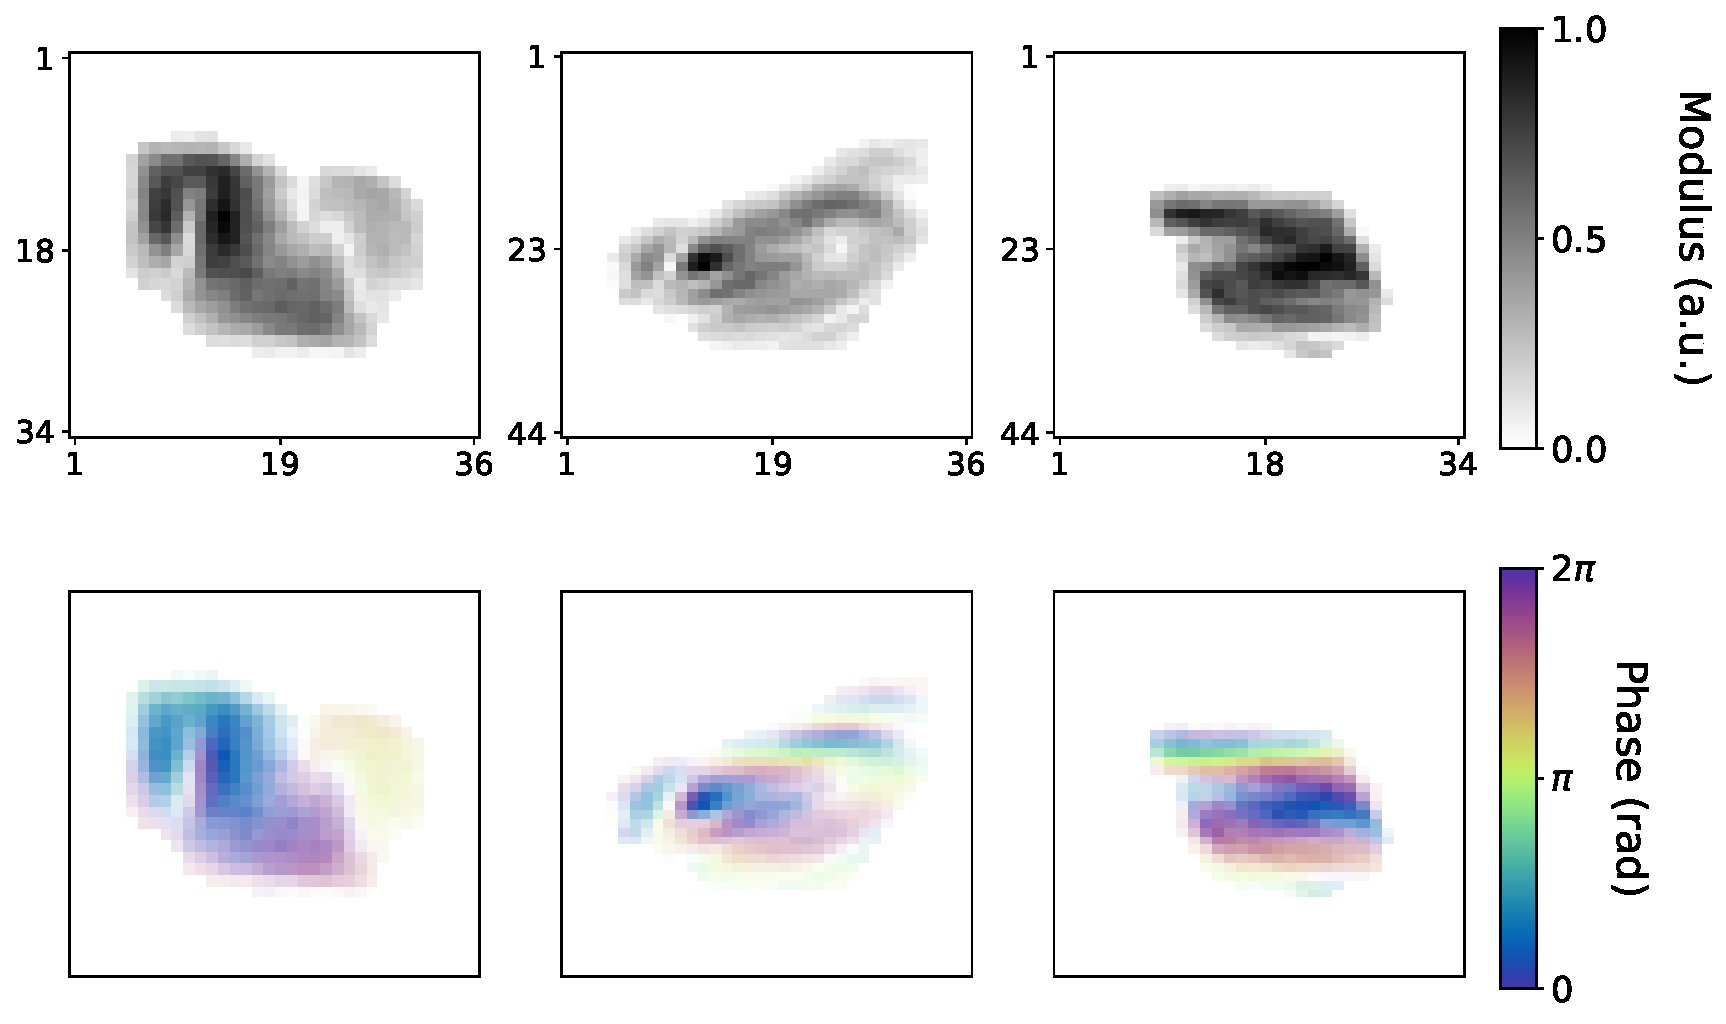
\includegraphics[width=\textwidth]{figures/AD/pynx_michael.pdf}
  \caption{Central slices for modulus (first row) and phase (second row) of the reconstruction obtained with the PyNX method.
           The presence of holes and inhomogeneous object's electron density suggests a poor quality reconstruction.}
  \label{fig:pynx_michael}
\end{figure}

\begin{figure}[H]
  \centering
  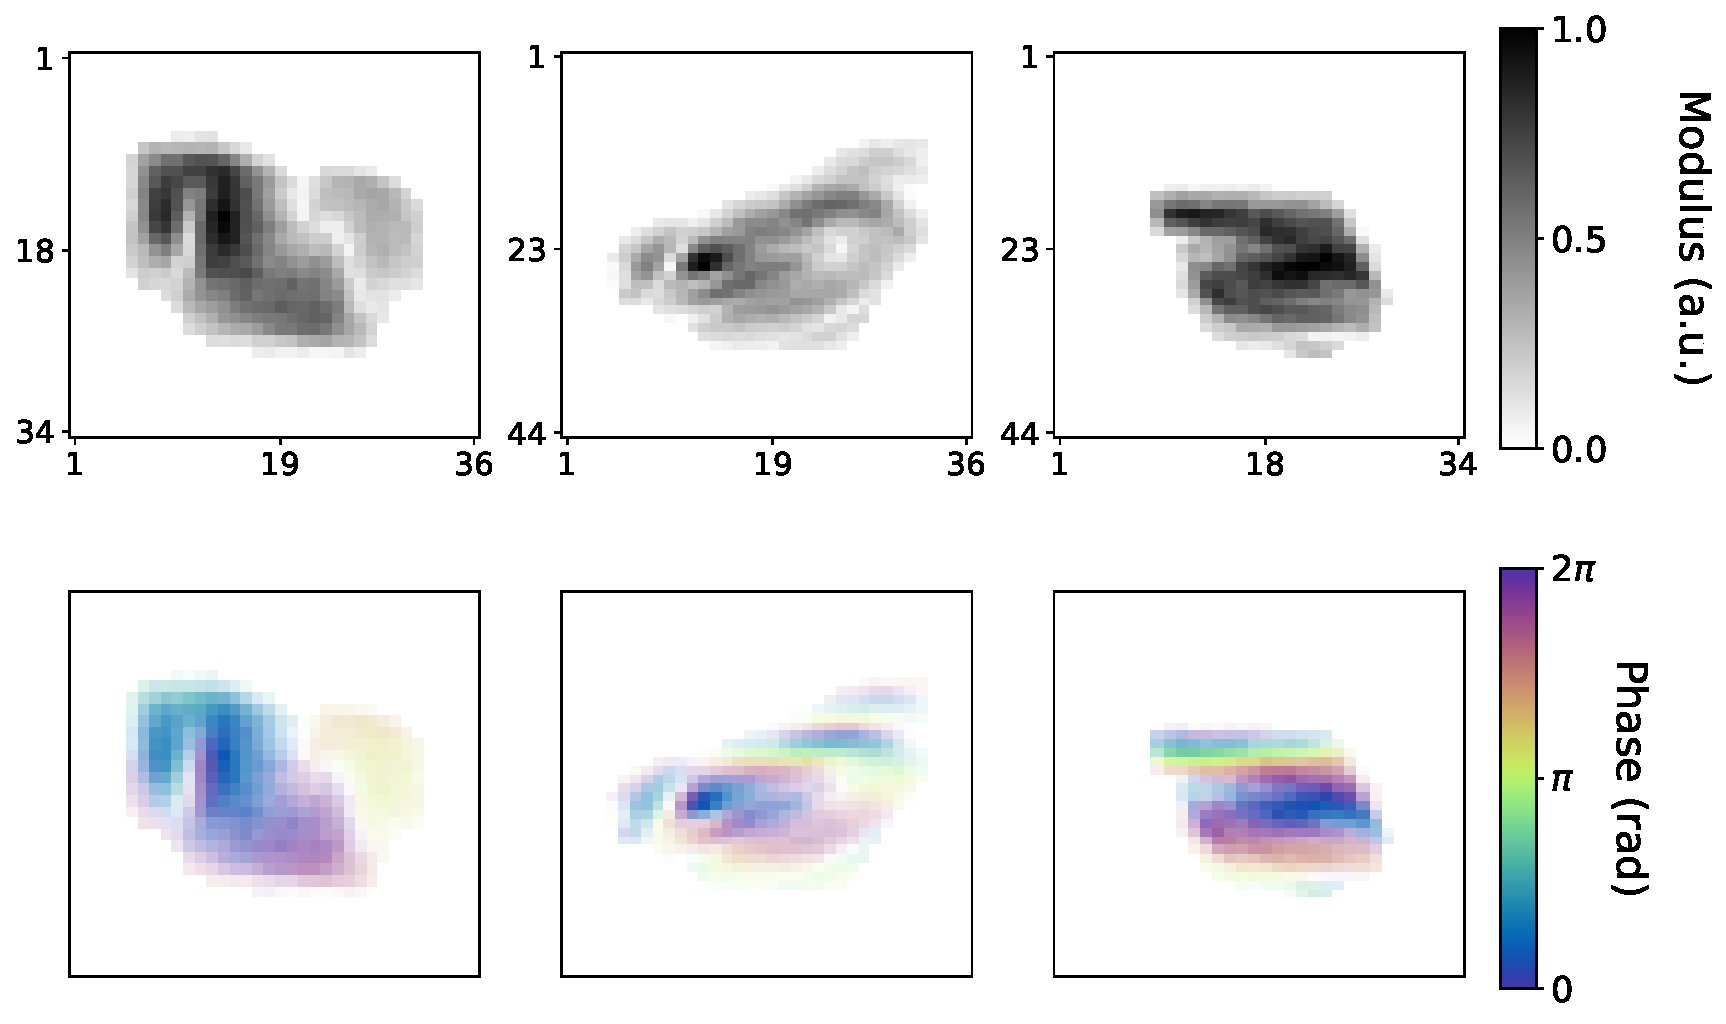
\includegraphics[width=\textwidth]{figures/AD/dl_pynx_michael.pdf}
  \caption{Central slices for modulus (first row) and phase (second row) of the reconstruction obtained with the DL + PyNX 
  method. Although the increased quality, the result cannot be considered a good reconstruction.}
  \label{fig:dl_pynx_michael}
\end{figure}

\begin{figure}[H]
  \centering
  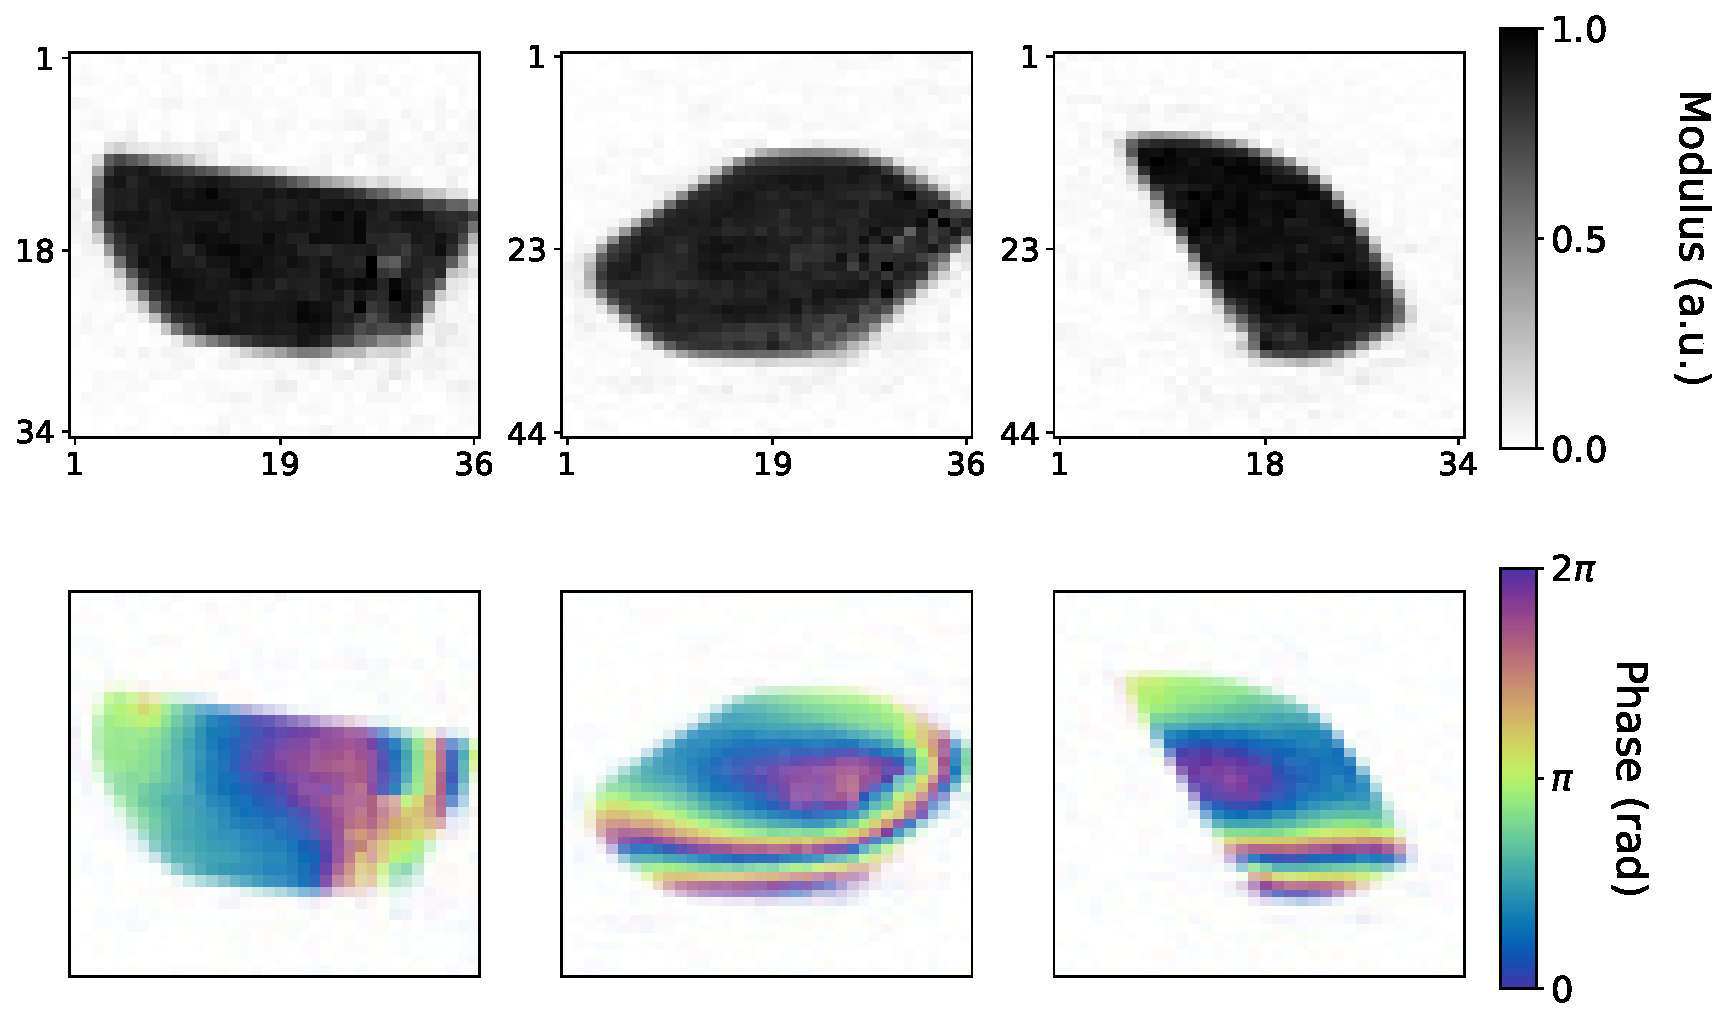
\includegraphics[width=\textwidth]{figures/AD/ad_michael.pdf}
  \caption{Central slices for modulus (first row) and phase (second row) of the reconstruction obtained with the AD method.
  The model converges to a reasonable result for Winterbottom shaped particle with visible high-strain given by the large phase ramp wrapped 
  multiple times.}

  \label{fig:ad_michael}
\end{figure}

\begin{figure}[H]
  \centering
  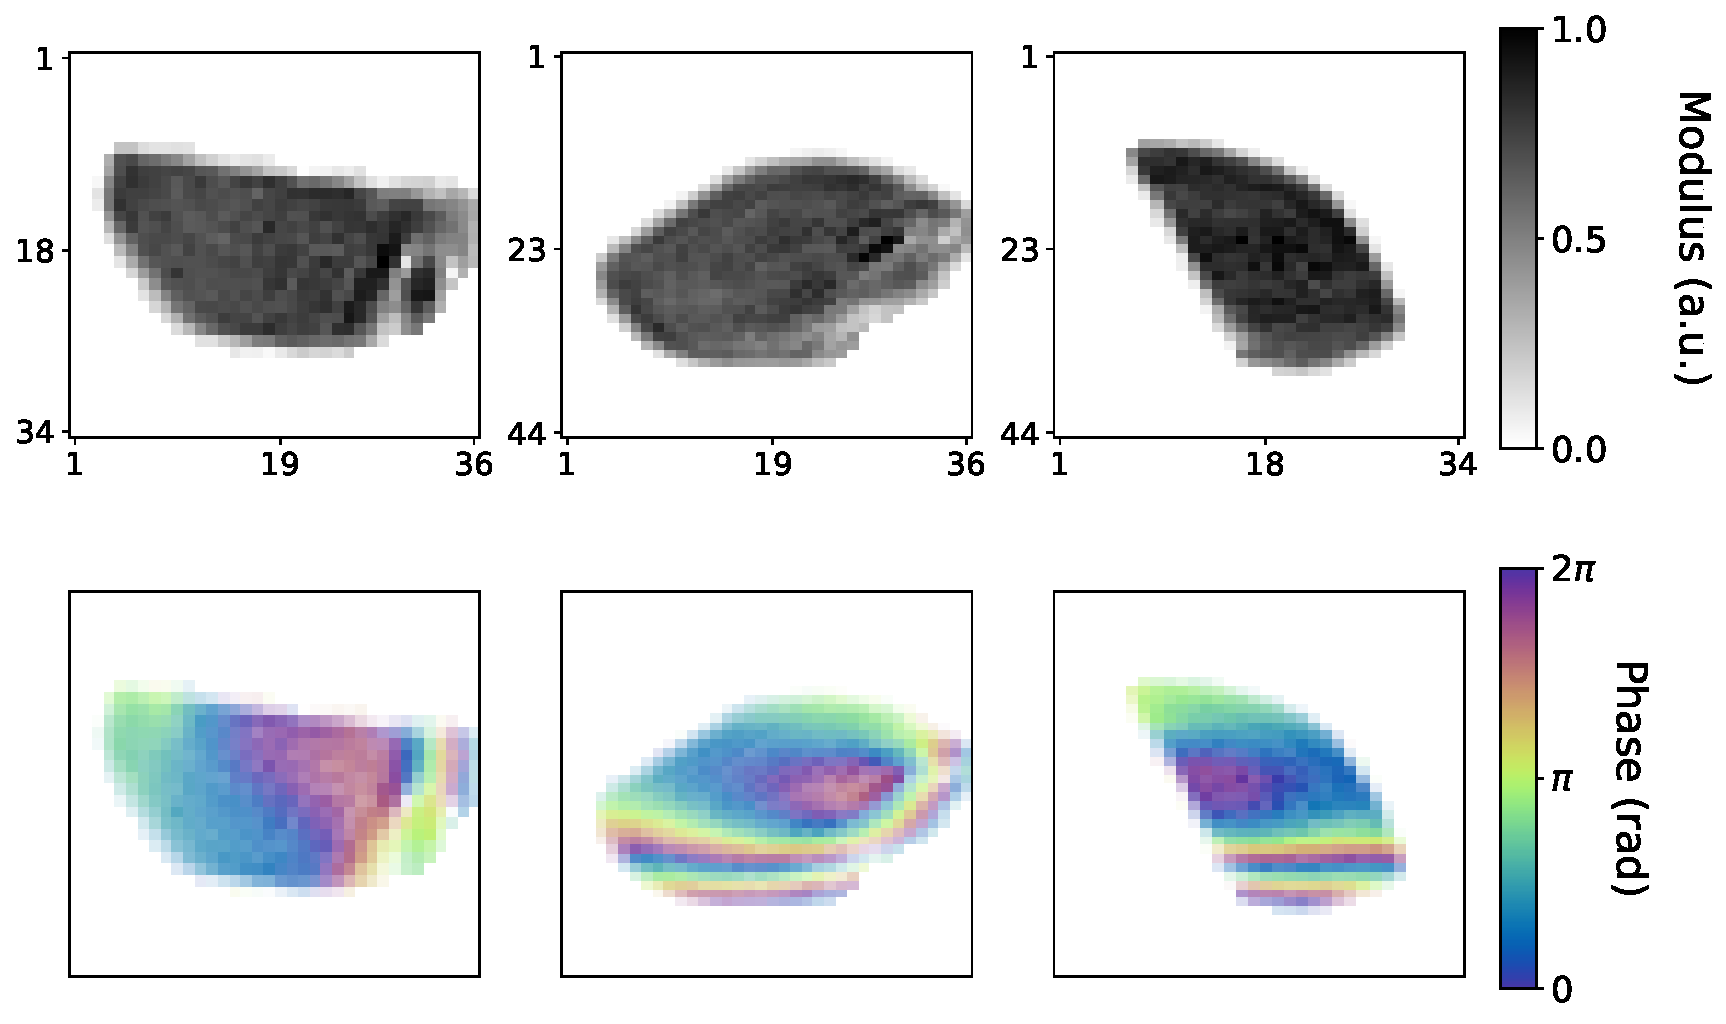
\includegraphics[width=\textwidth]{figures/AD/ad_pynx_michael.pdf}
  \caption{Central slices for modulus (first row) and phase (second row) of the reconstruction obtained with the AD + PyNX method.
  The 300 iterations of ER refinement do not alter the shape nor the phase found by the AD model, therefore validating the solution.}
  \label{fig:adpynx_michael}
\end{figure}

% DISLOCATIONS
\subsection{Hardly-invertible BCDI patterns with multiple dislocations}

In this paragraph another illustrative example is presented. This time a ... particle. 
The 4 different methods presented above are repeated here for this dataset in the same way and the results are shown in  
the following Figures \ref{fig:pynx_mouad} - \ref{fig:dl_pynx_mouad} - \ref{fig:ad_mouad} - \ref{fig:adpynx_mouad}. 

\begin{figure}[H]
  \centering
  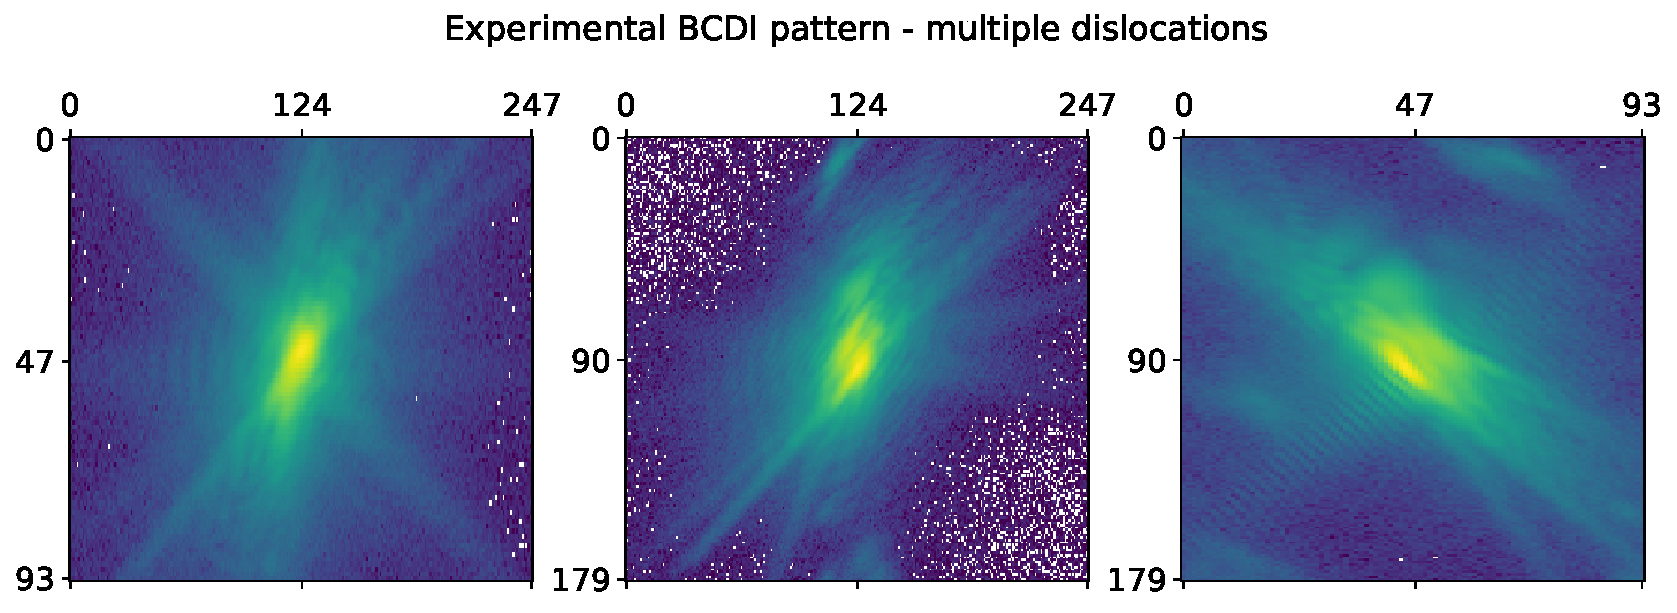
\includegraphics[width=\textwidth]{figures/AD/projections_mouad.pdf}
  \caption{Projections along the three axes of a dataset with multiple dislocations. }
  \label{fig:projectsions_mouad}
\end{figure}

\begin{figure}[H]
  \centering
  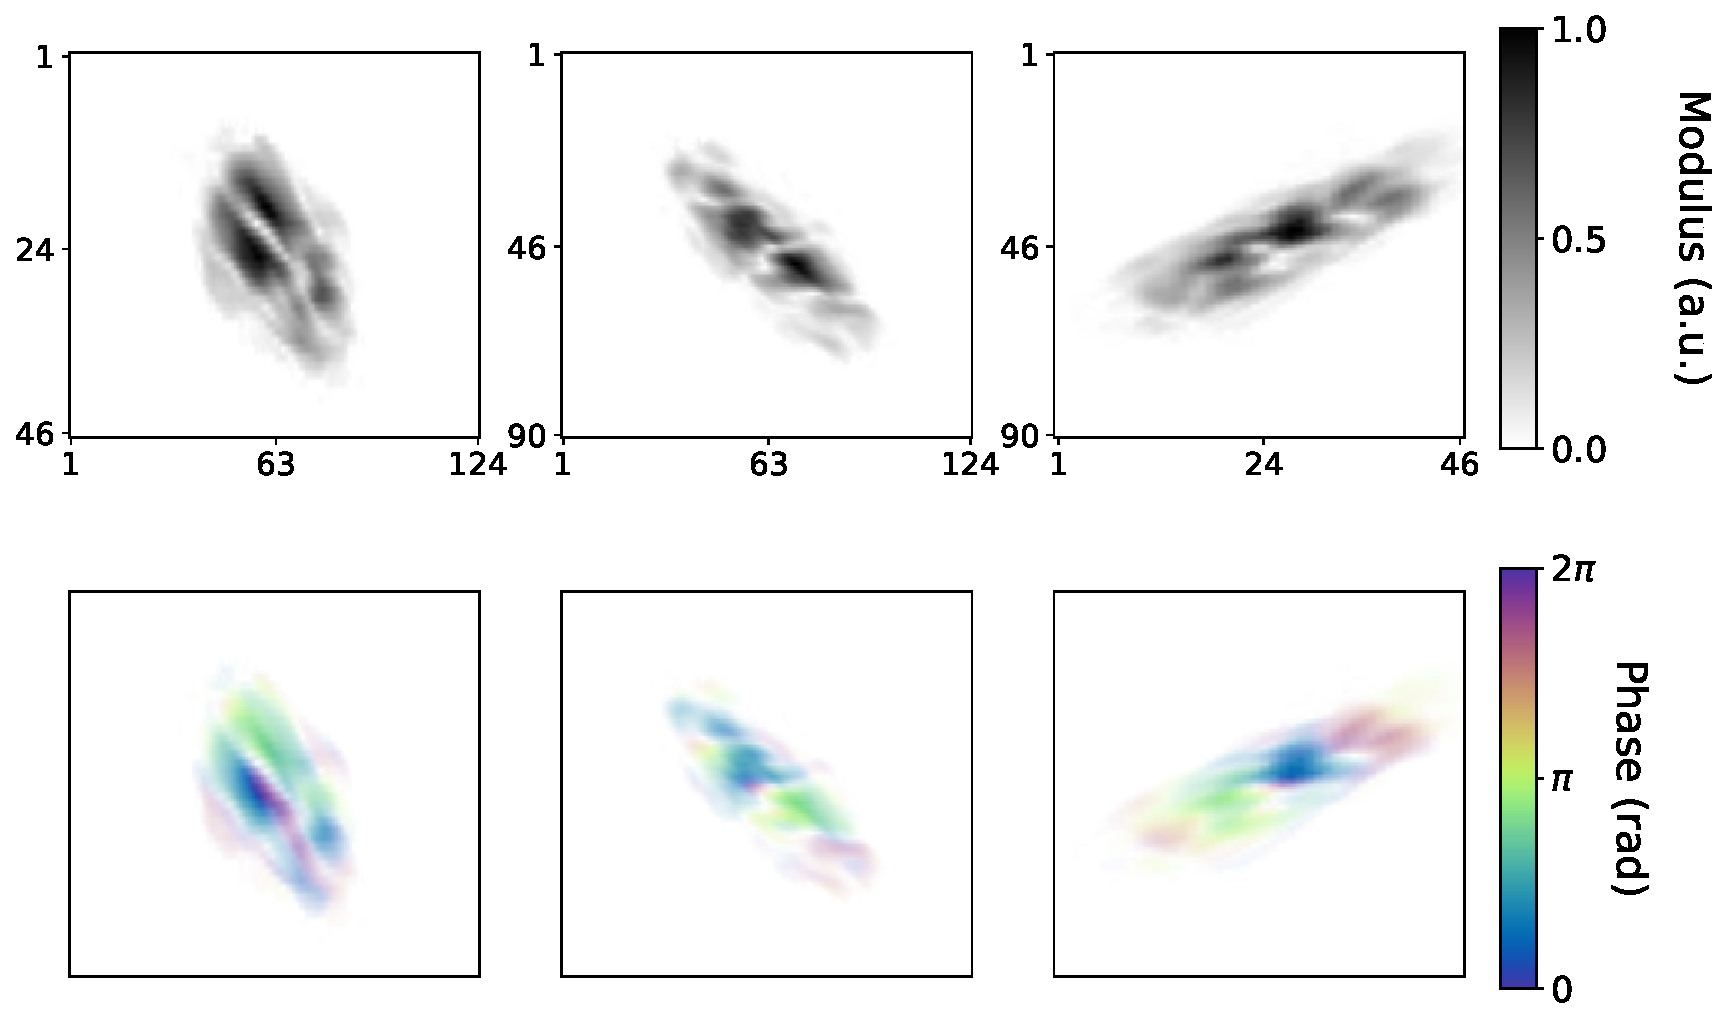
\includegraphics[width=\textwidth]{figures/AD/pynx_mouad.pdf}
  \caption{Central slices for modulus (first row) and phase (second row) of the reconstruction obtained with the PyNX method.
  The presence of holes and inhomogeneous object's electron density suggests a poor quality reconstruction. }
  \label{fig:pynx_mouad}
\end{figure}

\begin{figure}[H]
  \centering
  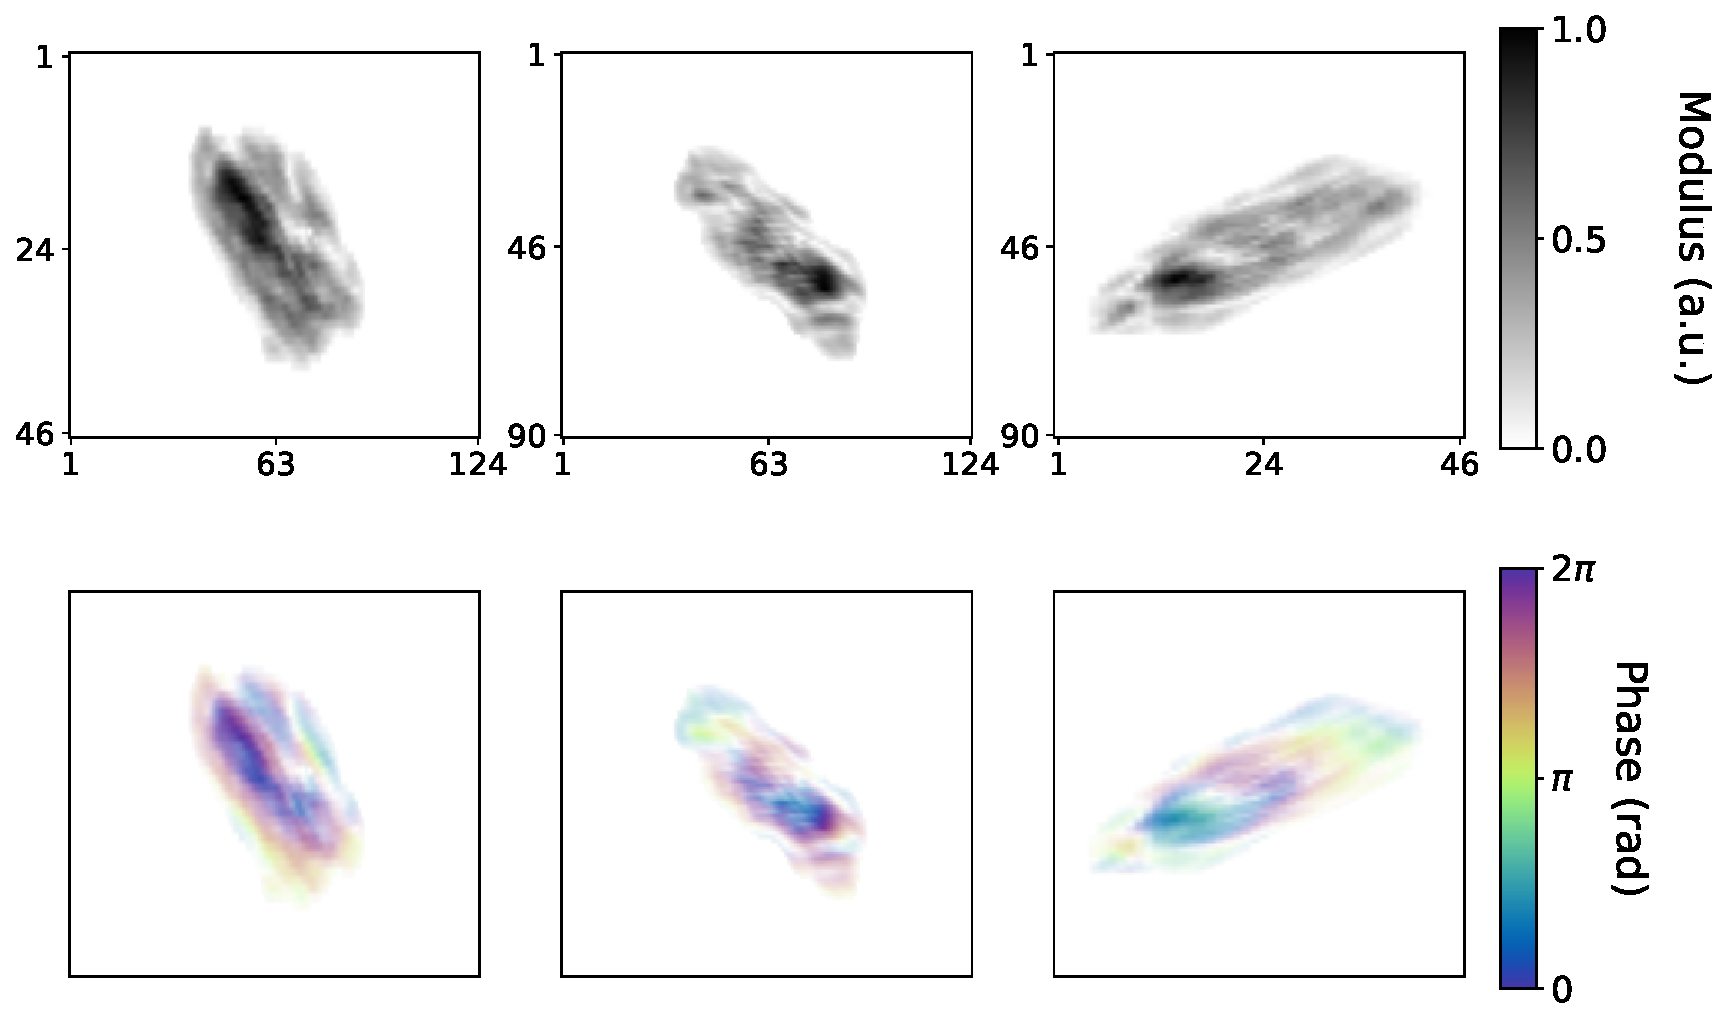
\includegraphics[width=\textwidth]{figures/AD/dl_pynx_mouad.pdf}
  \caption{Central slices for modulus (first row) and phase (second row) of the reconstruction obtained with the DL + PyNX 
  method. Here, a failure of the DL prediction is expected also because it hadn't been trained on datasets with dislocations. }
  \label{fig:dl_pynx_mouad}
\end{figure}


\begin{figure}[H]
  \centering
  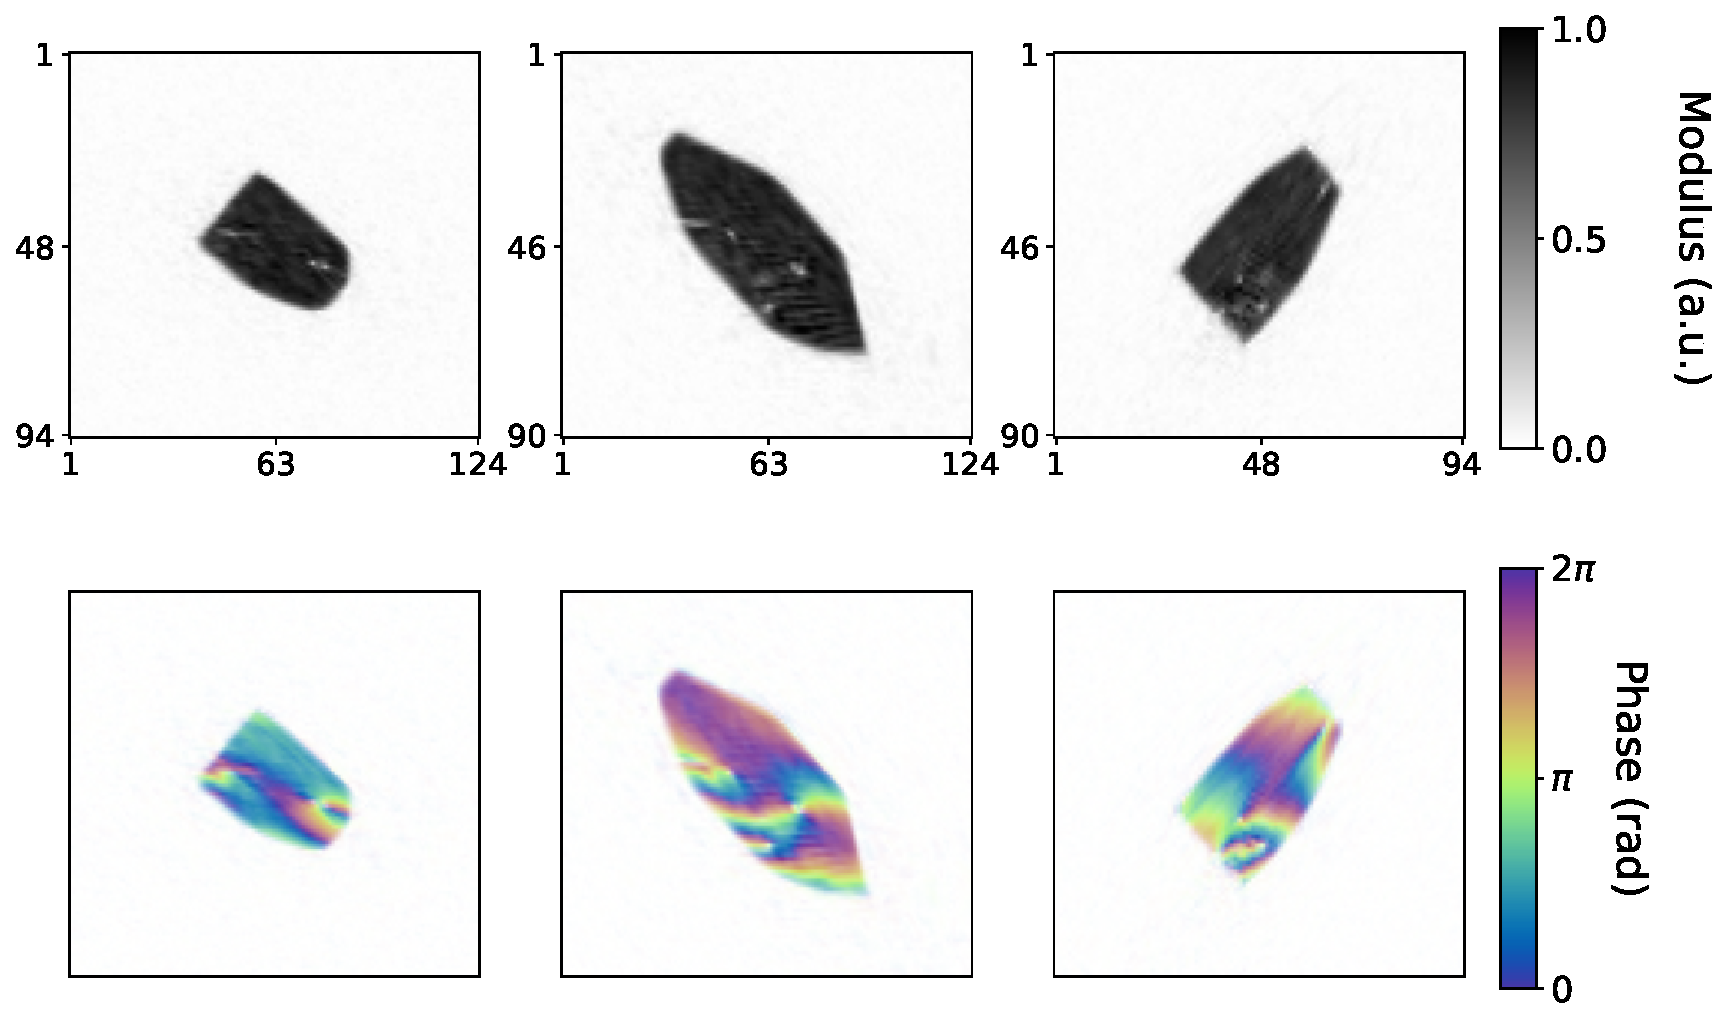
\includegraphics[width=\textwidth]{figures/AD/ad_mouad.pdf}
  \caption{Central slices for modulus (first row) and phase (second row) of the reconstruction obtained with the AD method.
  The AD model converges to a reasonably faceted crystal with several dislocations.}
  \label{fig:ad_mouad}
\end{figure}

\begin{figure}[H]
  \centering
  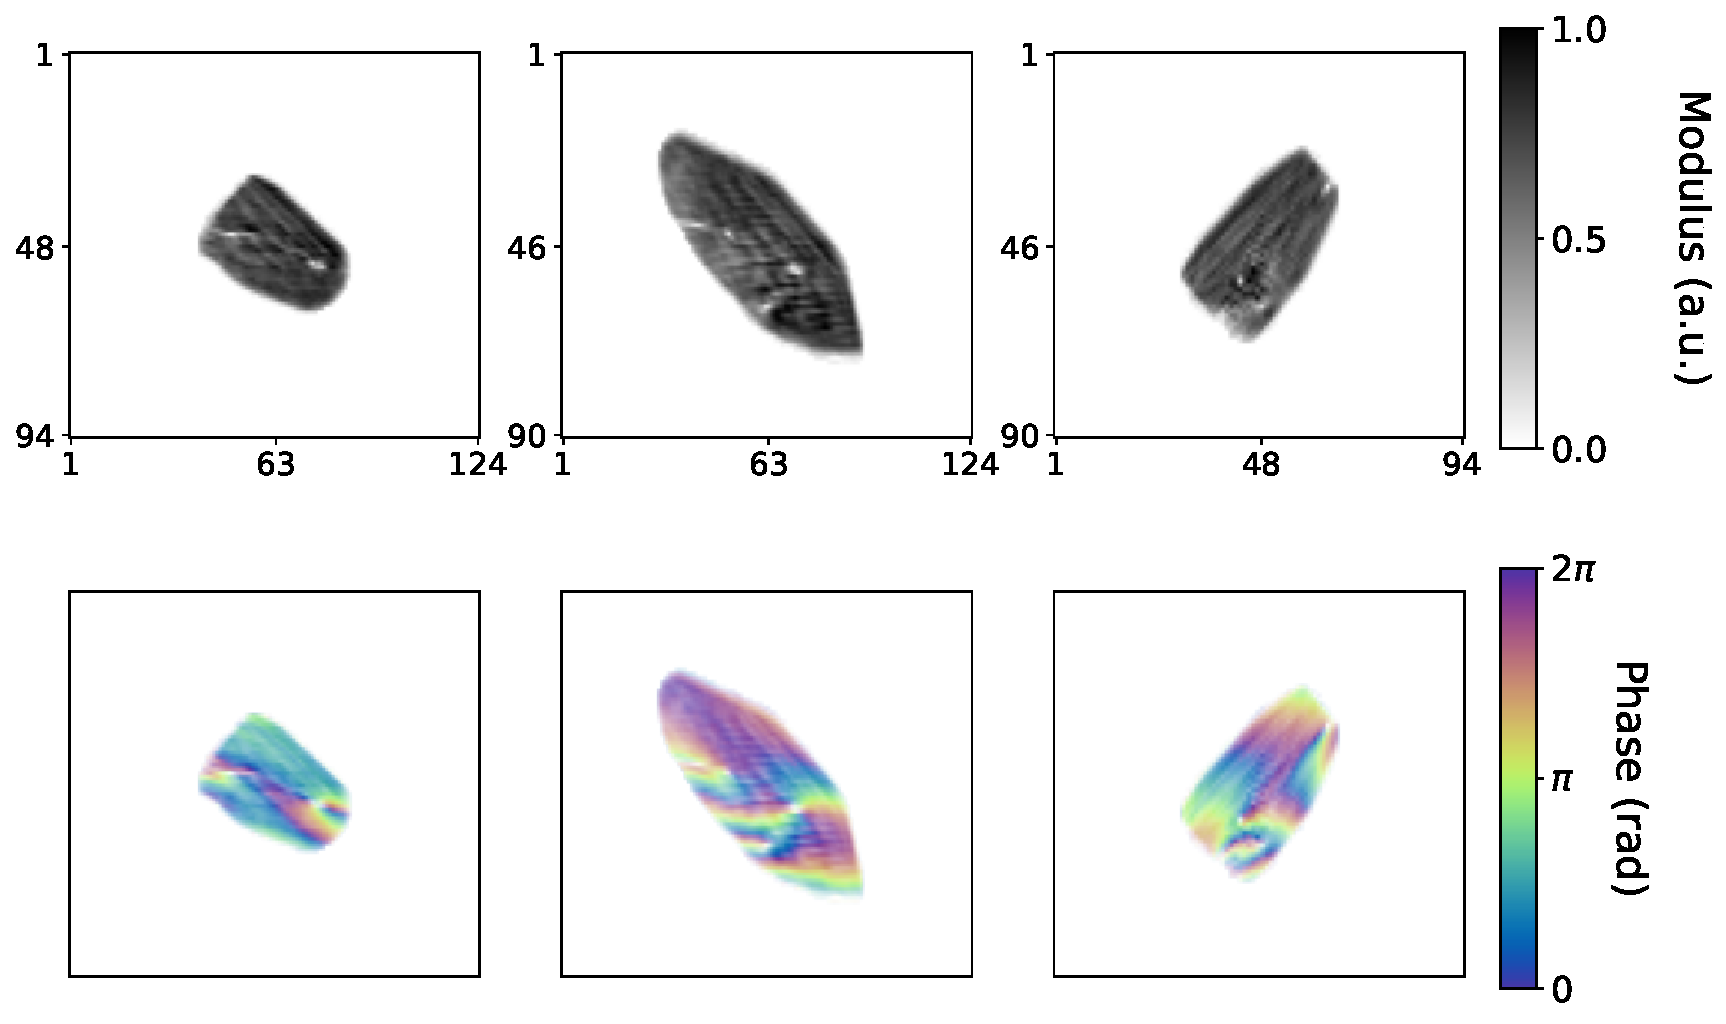
\includegraphics[width=\textwidth]{figures/AD/ad_pynx_mouad.pdf}
  \caption{Central slices for modulus (first row) and phase (second row) of the reconstruction obtained with the AD + PyNX method.
  The 300 iterations of ER refinement do not alter the shape nor the phase found by the AD model, therefore validating the solution.
  Some ripples appear instead in the objects' modulus and phase, probably caused by the presence of some neighbor crystals illuminated by the 
  x-ray beam, scattering on the same detector ROI (\textit{aliens}). }
  \label{fig:adpynx_mouad}
\end{figure}


\section{Conclusions}

In this chapter a novel PR method for BCDI based on a physics-informed AD model has been presented. The goal of this 
project was to explore GD-based methods for PR, aiming at resolving those difficult cases for which both conventional 
iterative algorithms and DL assisted methods struggle. To sum up, 
the major factors that made the model successful are here listed briefly: 
\begin{itemize}

  \item The efficient exact gradient calculation offered by the automatic differentiation, already identified by Jurling and 
  Fienup as potential alternative to alternating projections for PR, is today easily accessible and GPU accelerated by common 
  machine learning programming libraries like Tensorflow and PyTorch. This ingredient is fundamental for PR of 3D datasets 
  in competitive computational times, comparable to standard PR algorithms optimized for GPUs. 

  \item Being Fourier PR known to be sensitive to local minima, it is crucial to employ stochastic gradient descent 
  strategies. In particular, the ADAM optimizer combines the stochasticity of mini-batch optimization with adaptive 
  step-size tuning (eliminating the need to set a single learning rate for all parameters) and first and second order 
  moment estimation (thus providing both direction smoothing and per-parameter scaling), leading to more stable and 
  faster convergence. Once again this optimizer is already wrapped into a handy Tensorflow method. 

  \item The possibility to easily embed physical constraints in the forward model. In this case the prior knowledge on the 
  homogeneous and compactly supported nature of the crystal electronic density can be easily implemented with the half-spaces 
  method, thus restricting the solution space without need for additional regularization. In the same way, the Tucker 
  decomposition of the object's phase tensor facilitates the finding of physical solutions. 

  \item The multidimensional tensor-based computations typical of modern machine learning libraries make it straightforward 
  to extend the optimization to multiple parallel instances of the same phase retrieval problem, with only a modest 
  increase in computational time. The main limitation, however, lies in the substantial GPU memory requirements, as 
  this approach can be highly memory-intensive. To give some useful numbers, with the parameters shown in Table \ref{table:AD} 
  a GPU with 32GB of RAM can sustain the optimization of maximum 30 copies of a $64\times 64\times 64$ diffraction pattern. 

  \item The loss function definition gives the user high flexibility of implementing the most suitable metric for the 
  specific problem, allowing for parameter tuning during the optimization as well. In this case the MAE metric was found to be the 
  best one for the BCDI problem.  
  
\end{itemize}

This study has therefore shown that AD-based PR for BCDI is a valuable alternative to conventional or data-driven PR algorithms. 
It offers an additional tool that can extend the range of applicability of the BCDI technique to highly defective or strained 
crystals. Furthermore, it can be improved to include non-convex objects or separated ones (e.g. in case of twin boundaries) 
as well as different forward models beyond the kinematic approximation. 
